\documentclass[journal,10pt]{IEEEtran}
\usepackage{amsmath}
\usepackage{graphicx}
\usepackage{float}
\usepackage{comment}
\usepackage{setspace}
\usepackage{caption}
\usepackage{hyperref}
\usepackage[T1]{fontenc}
\doublespacing
\title{ 
\begin{huge}
\textbf{L2 Design Feasibility Report: Electric Skateboard} 
\end{huge} }
\author{Toby Ashton, Jacob Black, Hugo McCartney, Haydn Lisk, Edward Street, Sam Sutcliffe}
\begin{document}
\maketitle
\tableofcontents
\newpage
\section{Executive Summary}
        This project concerns the design and construction of an electric skateboard based on a traditional longboard.
\section{Introduction}
        This project's scope consists of designing an electric skateboard capable of carrying a large male for daily transport. A longboard was supplied which will be modified to produce the final product. 
\section{Board}
    \subsection{Overview}
        The board provided was a 'Mindless Raider I model (34’’ x 8’’)’\cite{boardModel}. The deck was modelled in SOLIDWORKS and assembled with a library model of the trucks \cite{trucksCAD} - this allowed a Finite Element Method (FEM) analysis to be performed. Material properties were taken for maple wood, as it is the main board material. Fig \ref{fig:Board_Rendering} shows a rendering of the final concept \cite{shoesCAD}. 
        \begin{figure}[H]
                \centering
                \scalebox{0.25}{\includegraphics{"./Board/Skateboard_Rendering".png}}
                \caption{
                Rendering of Skateboard}
                \label{fig:Board_Rendering}
            \end{figure} 
    \subsection{Component Arrangements}
        Several arrangement options for the electrical components were explored, subject to the following limiting factors:
        \begin{itemize}
            	\item Ground Clearance
            	\item Transmission Efficiency
            	\item Balance 
            	\item Rider Comfort
            \end{itemize}
        \begin{figure}[H]
                \centering
                \scalebox{0.25}{\includegraphics{"./Board/Concept_A".png}}
                \caption{Concept A}
                \label{fig:ConceptA}
            \end{figure} 
        \begin{figure}[H]
                \centering
                \scalebox{0.15}{\includegraphics{"./Board/Concept_B".png}}
                \caption{Concept B}
                \label{fig:ConceptB}
            \end{figure}  
        \begin{figure}[H]
                \centering
                \scalebox{0.15}{\includegraphics{"./Board/Concept_C".png}}
                \caption{Concept C}
                \label{fig:ConceptC}
            \end{figure} 
        \begin{figure}[H]
                \centering
                \scalebox{0.15}{\includegraphics{"./Board/Concept_D".png}}
                \caption{Concept D}
                \label{Fig:ConceptD}
            \end{figure} 
        \begin{figure}[H]
                \centering
                \scalebox{0.15}{\includegraphics{"./Board/Concept_E".png}}
                \caption{Concept E}
                \label{Fig:ConceptE}
            \end{figure}
    \subsection{Structural Analysis}
        %Rider load was assumed to total 1100N, applied over two 10cmx10cm areas at appropriate positions on the board. An additional load of 80N was applied at the centre of the wheelbase to model the weight of the electrical components.The simulation computed the maximum Von-Mises stress to be approximately 31.69MPa, located at the joint between the truck and the board, as shown in the figures below.
        \begin{figure}[H]
            \centering
            \scalebox{0.35}{\includegraphics{"./Board/Stress_Analysis_Top".png}}
            \caption{FEM Von Mises Stress Analysis of Top Surface of the Board
            }
            \label{fig:stressTop}
        \end{figure}
        \begin{figure}[H]
            \centering
            \scalebox{0.35}{\includegraphics{"./Board/Stress_Analysis_Bottom".png}}
            \caption{FEM Von Mises Stress Analysis of Bottom Surface of the Board
            }
            \label{fig:stressBottom}
        \end{figure}
        %Comparing this to the yield strength of maple wood, approximately 65.5MPa \cite{materialProperties}, a Factor of Safety value of approximately 2.1 was calculated. A further simulation was performed with the rider's load scaled up by this FOS, and the load located at a single 10cmx10cm area at the centre of the wheelbase. Maximum displacement was calculated as approximately 18.19mm (shown below). 
        \begin{figure}[H]
                \centering
                \scalebox{0.4}{\includegraphics{"./Board/Displacement".png}}
                \caption{Displacement Contour of Board When Put Under Maximum Loading
                }
                \label{fig:Displacement}
            \end{figure}
        %With the unloaded board height of 110mm, this allows a minimum ground clearance of approximately 91.8mm - this was considered acceptable as the electrical components will have a max height of 45.9mm considering a FOS of 2.
    
\section{Powertrain}
    \subsection{Transmission}
        \subsubsection{Gearing}
            Gears provide a vast array of gear ratios but the large range of output speeds of motors makes large gear ratios unnecessary.
        \begin{figure}[H]
            \centering
            \scalebox{0.125}{\includegraphics{"./Drivetrain/Images/Drivetrain1Lab".png}}
            \caption{Arrangement with gears}
            \label{fig:DrivetrainChain}
        \end{figure}
        \subsubsection{Hub Motor}
            Hub motors are contained in the wheels of the skateboard, offering many advantages including quietness, low maintenance and sleek appearance.
            However as they have no gearing and have limited space, they provide less torque than other drives. %\[cooling?, wheel customization, ride- thin polyurethane]
        \subsubsection{Chain}
            Using a chain drive is the most efficient way to transmit power amongst the options covered, with a typical efficiency of 98\%. \cite{Mechanical_Power_Transmission} However, high maintenance is required due to the need for lubrication to prevent wear and corrosion. 
        \subsubsection{Belt}
            Due to the elasticity of toothed rubber belts, this option provides low noise and vibration, and efficient power transmission. Furthermore, they require relatively low maintenance and have a long lifespan making this preferable.
        \begin{figure}[H]
            \centering
            \scalebox{0.14}{\includegraphics{"./Drivetrain/Images/Drivetrain2Lab".png}}
            \caption{Arrangement with Belt or Chain}
            \label{fig:Drivetrain2}
        \end{figure}
        \begin{figure}[H]
            \centering
            \scalebox{0.13}{\includegraphics{"./Drivetrain/Images/Drivetrain3Lab".png}}
            \caption{Arrangement with Belt attached to trucks}
            \label{fig:Drivetrain3}
        \end{figure}
        
    \subsection{Motor}
        \subsubsection{Required Parameters}
        The main requirements of the motor at 8$ms^{-1}$, with a slope of 10$^{\circ}$ and 1$ms^{-2}$ acceleration using equations bellow are:
        \begin{itemize}
        	\item Size- The motor must fit under the board and be relatively lightweight
        	\item Torque- 13Nm at the wheel 
        	\item Speed- The $K_{v}$ motor parameter should be 250 eqn
        	\item Power- 2000w assuming no acceleration uphill at 8$ms^{-1}$
        \end{itemize}
        \begin{gather}
            F = F_{Rolling Resistance} + F_{Acceleration} + F_{Gravity}\\
            F_{Acceleration} = Mass \times Acceleration\\
            F_{Gravity} = Weight \times sin(Slope Angle)\\
            F_{Rolling Resistance} = 4.64N\\
            Torque = F_{Total} \times R_{Wheels}\\
            Wheel RPM = \frac{Velocity (ms^{-1})}{Radius}\times \frac{60}{2\pi}\\ 
            Motor Power = \frac{F_{Total} \times Velocity (ms^{-1})}{Efficiency}
        \end{gather}
        \subsubsection{AC Motor}
            AC induction motors have excellent efficiency, reliability and durability. However, using DC supply would require a variable frequency inverter to produce AC speed control, and particularly with single phase induction motors the staring toque is very low, an issue for hills. 
        \subsubsection{DC Brushed Motor}
            Using a commutator allows a motor to be run from a DC supply but using carbon brushes adds a large amount of friction and varying the speed of this type of motor is harder, especially if two motors were implemented and run synchronously.
        \subsubsection{DC Brushless Motor}
            With an electronic speed controller a motor can be run from a DC supply with speed control and without a commutator meaning less friction so greater efficiency, longer lifespan and reduced weight for the same output power. This motor family also gives a large staring torque, enabling the board to accelerate quickly at low speeds \cite{AC_Motor}. For these reasons it was decided a DC brushless motor would be used.
    \section{Battery}
    A compact and quickly rechargeable battery is required. A supply rail of 24V is common for consumer electronics and will not require high voltage safety precautions. Battery charge capacity (amp-hours) and energy capacity are used roughly interchangeably due to the constant supply voltage for ease of calculation but will be annotated with the units strictly.
        \subsubsection{Capacity}
            The larger a battery network's capacity, the heavier and more expensive it becomes.Two main considerations regarding required capacity are range and lifespan. Range is be determined by average daily usage (a 1.5 km round trip between Butler and Science sites, (Fig. \ref{fig:route}) and expected charge frequency (assumed once a week).
            \begin{figure}[H]
                \centering
                \scalebox{0.5}{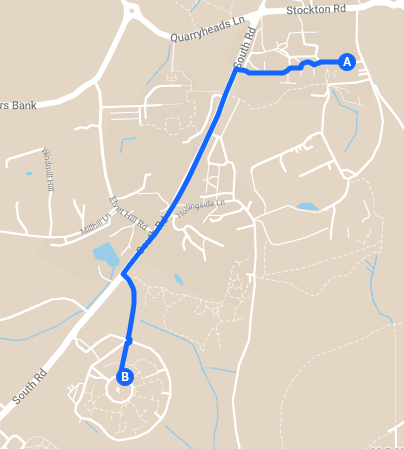
\includegraphics{./Battery/RouteAnalysis/Route.png}}
                \caption{Typical Daily Route}
                \label{fig:route}
            \end{figure}
            Extra energy considerations will be needed for the range as there is a relatively large height change throughout the route.
            Elevation and gradient variations can be seen in the graphs below, with data sourced from various GPS public databases via an online website \cite{GPSDatabase}.
            Fig \ref{fig:elevation} shows the elevation of the route and makes a difference for the maximum capacity needed.
            Fig \ref{fig:gradient} shows the gradient of this route, which will effect the maximum torque required.
            \begin{figure}[H]
                \centering
                \scalebox{0.5}{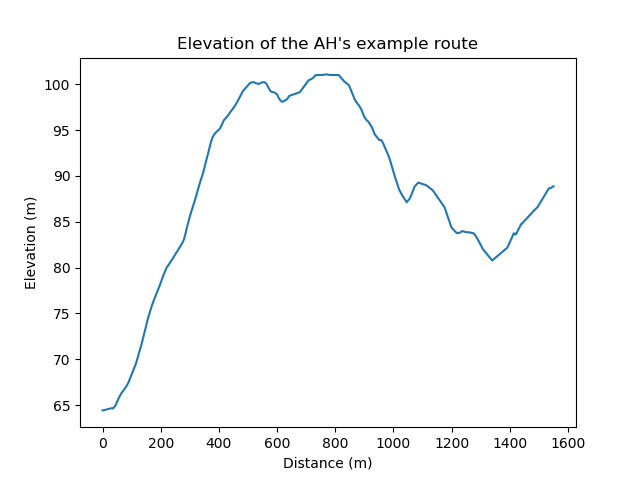
\includegraphics{./Battery/RouteAnalysis/elevation.png}}
                \caption{Elevation of Route}
                \label{fig:elevation}
            \end{figure}
            \begin{figure}[H]
                \centering
                \scalebox{0.5}{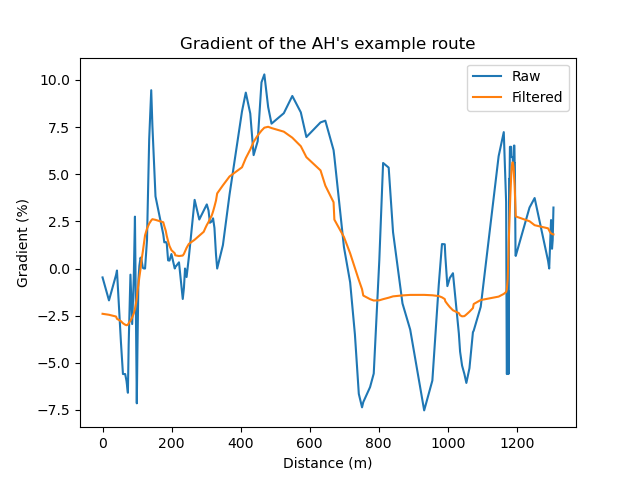
\includegraphics{./Battery/RouteAnalysis/grad.png}}
                \caption{Gradient of Route}
                \label{fig:gradient}
            \end{figure}
            Total elevation change consists of 50m uphill and 25m down (heading south). Energy requirements are modelled as a simple vehicle hoist to give an estimate (Energy = $mg\Delta h$). Total vertical ascent over the trip is 75m, so approximately 90kJ (25Wh) more energy will be required than with a flat route.
        \subsubsection{Energy Requirement Estimates}
            10Wh/mile (based off electric bike: 12Wh/mile)
            Total Energy of Journey (including vertical): 37Wh
            Per Week Consumption: 5 x 37.5Wh = 185Wh
            -Absolute Minimum Required Capacity of 185Wh
        %\subsubsection{Charging}
            %Charging the battery is a complex concern, as specific charging circuits are required to prevent damage to the system. This is particularly true of modern batteries due to the large release of heat associated with large energy transfers.
        \subsubsection{Lifespan}
            \begin{figure}[H]
                \centering
                \scalebox{0.5}{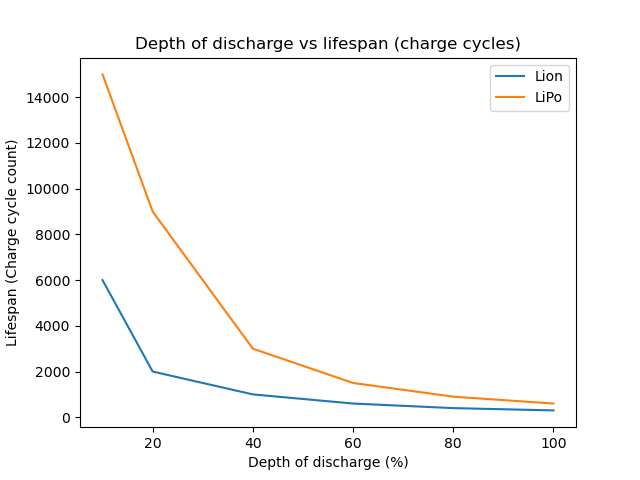
\includegraphics{./Battery/ChargeCycles/DoD.png}}
                \caption{Lifespan vs DoD (Depth of Discharge)}
                \label{fig:DoD}
            \end{figure}
            \cite{BatteryLifespan} 
            \ref{fig:DoD} illustrates the superior lifespan at comparable discharge depths.
            Lithium-ion batteries have a life cycle of approximately 800 cycles at 50\% DoD, whereas Lithium Polymer cells perform better at approximately 2000 charges at the same DoD - we will be using LiPo for this reason. Given that the capacity required at 100\% DoD is 185Wh, a 370Wh capacity is needed to achieve 50\% DoD for a full use.
        \subsubsection{Rate of Charge}
            Lithium polymer batteries are charged at a constant rate until they reach near capacity at which they slow down and shut off. Recharge time has to have a lower bound percentage. General guidelines suggest that the charge rate should not exceed 1C [Pushing the total amp hours in one hour] to ensure optimal battery life. Ideally, the battery will charge from 50\% empty to full overnight. This will be achievable at a sub 1C rate [15 amps], which allows it to recharge from consumer wall sockets.
        \subsubsection{Battery Size}
        Battery volume and weight are limiting factors wrt. capacity. Volume affects how the components can be arranged on the board, while weight directly impacts the board's performance.    
        Using the calculated capacity the volume and mass can be calculated with the volumetric \& graviometric density. Using values from \ref{fig:Battery Size}, the volume comes to about 1.2 Litres with a mass of 2.3Kg.
            \begin{figure}[H]
                \centering
                \scalebox{0.40}{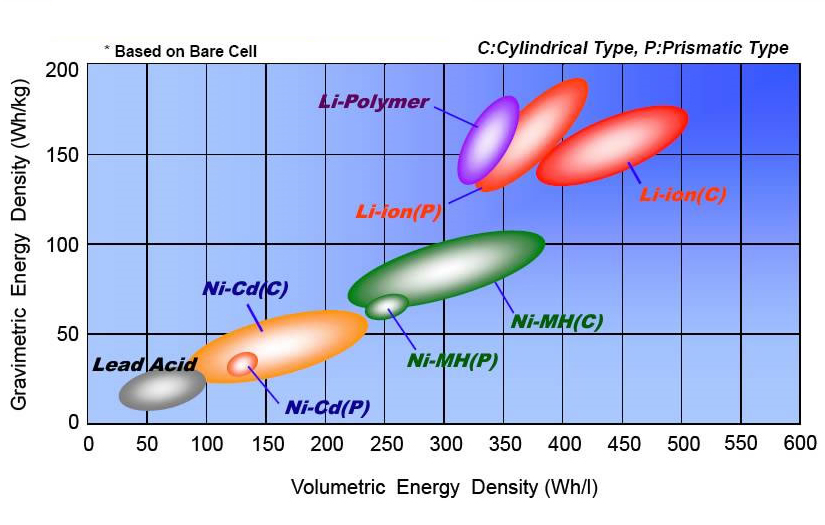
\includegraphics{./Battery/Density.png}}
                \caption{Ragone Plot \cite{BatteryDensity}}
                \label{fig:Battery Size}
            \end{figure}
\section{Trucks}
    \subsection{Operating Terrain}
        The board will be operating over mostly smooth surfaces - however, disturbances such as uneven patches of road, litter and debris will still be present. At high speeds, low frequency oscillations (4-10Hz, called 'speed wobble') build and begin to impede rider control. A suspension system is thus required to minimise these effects.
    %\subsection{Speed Wobble}
        %This phenomenon consists of unpredictable vibrations (approx. 4-10Hz) induced in the board when running at high speed – if neglected, these oscillations could directly affect the user’s ability to control the board, reducing rider comfort and potentially resulting in injury. 
    \subsection{Potential Solutions}
        Buying existing truck suspension systems would free up development time, however due to availability constraints, a bespoke design may be necessary.
        Several patented designs exist, as shown in figures \ref{fig: Spring Idea}, \ref{fig: Seperate Spring Idea} and \ref{fig: Hanger Idea}. Fig.\ref{fig: Spring Idea} shows an ideal solution, with the decision to purchase or manufacture being dependent on labour and budget constraints.
        \begin{figure}[H]
            \centering
            \scalebox{0.2}{\includegraphics{"./Wheels/Spring Idea".png}}
            \caption{Credits: Seismic Skate}
            \label{fig: Spring Idea}
        \end{figure}
        \begin{figure}[H]
            \centering
            \scalebox{0.2}{\includegraphics{"./Wheels/Seperate Spring Idea".png}}
            \caption{Credit: US Patent 4,176,850 'SKATEBOARD TRUCK WITH INDEPENDENT WHEEL SUSPENSION'}
            \label{fig: Seperate Spring Idea}
        \end{figure}
        \begin{figure}[H]
            \centering
            \scalebox{0.35}{\includegraphics{"./Wheels/Hanger Idea".png}}
            \caption{Credit: Avenue Trucks}
            \label{fig: Hanger Idea}
        \end{figure}
\section{Wheels}
    \subsection{Overview}
        Various factors affect the wheel design – rolling resistance is affected by the wheel and bearing materials, with torque transferred dependent on the radii and material of the driven wheels.
    \subsection{Wheel Materials}
        Longboard wheels are typically made from polyurethane, which achieve a $\mu_{rolling}$ in the range 0.04-0.08 \cite{wheel_data}. While this is sufficiently small to provide low rolling resistance (see calculations below), polyurethane only provides a $\mu$-static of ~0.2, limiting the torque that can be transferred to the road. This can be improved by using rubber for the driven wheels as rubber achieves a $\mu$-static in the range of 0.35-0.45, providing an increase in torque transmitted of 75-125\%.
    \subsection{Bearing Materials}
        Longboard bearings come in three different material families: steel, titanium and ceramic. Ceramic (Silicon Nitride) has a Brinell hardness 1479 $kg/mm^{2}$ \cite{ceramic_data1}, approximately 640\% greater than AISI-52100 steel \cite{steel_data} and ASTM-7 Titanium \cite{titanium_data}, leading to reduced energy loss from elastic deformation.  However, Silicon Nitride exhibits a yield strength of 170MPa \cite{ceramic_data2}: approximately 64\% less than steel and titanium. Ceramic is thus inadvisable as the board will be used in an environment where it is expected to suffer shocks. Additionally, ceramic bearings cost significantly more than steel and titanium, the former often in the \$90-\$150 range, as opposed to \$15-\$20 and \$30 for steel and titanium respectively. As steel and titanium perform similarly, the latter’s corrosion resistance suggests that it is the optimal type as less maintenance will be required. 
    \subsection{Wheel Dimensions}
        Longboard wheels vary in diameter between 60-100mm with a contact-patch width of approx. 30mm. Larger wheel radii provide greater top speed and smoother ride, with smaller radii producing greater mechanical advantage. 
        Wheel diameter is selected to provide the desired torque when driven by the chosen motor.
        %Depending on the output of the motor and the required road-torque, the appropriate wheel size can be selected.
    \subsection{Estimates of Rolling Resistance}
        \begin{equation*}
        \resizebox{\columnwidth}{!}{%
            $F_{resistive} = (\mu _{static}  -  r_i sin(\alpha) \cos(\arcsin(\frac{r_f}{r_i}))  +  r_f cos(\alpha)(\frac{F_{load}}{r_o – r_i})$%
        }
        \end{equation*}
    $Static
    \\*F_{res-rubber} \approx 10.98N	
    \\*F_{res-polyurethane} \approx 4.88N
    \\*F_{res-total-static} = 2 F_{res-rubber} + 2 F_{res-polyurethane} = 31.72N 
    \\*Dynamic
    \\*F_{res-rubber} \approx 0.37N	
    \\*F_{res-polyurethane} \approx 1.95N
    \\*F_{res-total-dynamic} = 2 F_{res-rubber} + 2 F_{res-polyurethane} = 4.64N$
    \\*\cite{Combined_Resistance} 
    
\section{Control}
    \subsection{Overview}
    	Complex electronic systems will almost always require a control unit to operate them.
    	Three aspects of control must be designed for; the user interface, battery management, and motor/drive train control.
    	In this application, the one-off nature of the product lends itself to use a micro-controller for control, rather than bespoke hardware.
    	This is due to the ease of altering functionality, and the high volume of support documentation for these units.
    	Due to time and budget constraints, it may prove more effective to use existing circuit modules than implementing a bespoke design.
    \subsection{User Interface}
        \begin{figure}[H]
            \centering
            \scalebox{0.2}{\includegraphics{"./Control/Boosted Remote Labelled".png}}
            \caption{Market Leader's Remote Control}
            \label{fig:Boosted Remote}
        \end{figure}
        \begin{figure}[H]
            \centering
            \scalebox{0.2}{\includegraphics{"./Control/Pressure Pads
            Labelled".png}}
            \caption{Dual Pressure Pad Control}
            \label{fig:Pressure Pads}
        \end{figure}
            
    	\subsubsection{Throttle Control}
    	    To ride safely, the user requires rapid and intuitive speed selection.
    		The market leader utilises a handheld wireless controller (as shown Fig.\ref{fig:Boosted Remote} \cite{BoostedRemote}) which also relays status information to the rider.
    		A potential solution to this is a dual pressure pad control system, pictured in Fig.\ref{fig:Pressure Pads} \cite{PressurePads}.
            
    	\subsubsection{Status Meters}
    		The rider must know the remaining range/time of the board. The current market leader uses an array of LEDs on its controller for status information. This can be improved by using 7 segment displays or a small LCD, allowing for quantitative data to be shown to the rider. (shown in Fig.\ref{fig:7 seg} \cite{7seg} and Fig.\ref{fig:LCD} \cite{LCD}).
    		
    	\begin{figure}[H]
            \centering
            \scalebox{0.4}{\includegraphics{"./Control/7 Segment Labelled".png}}
            \caption{7 Segment Displays}
            \label{fig:7 seg}
        \end{figure}
    	\begin{figure}[H]
            \centering
            \scalebox{0.4}{\includegraphics{"./Control/LCD Labelled".jpg}}
            \caption{Arduino LCD}
            \label{fig:LCD}
        \end{figure}
    \subsection{Battery Management}
    	Care must be taken to ensure that during normal operation the battery is charged safely.
    	This includes tracking the number of charge cycles, as well as the temperature, with a view to disabling the system if the battery is no longer in a safe state.
    	
    		%General guidelines suggest charging at no faster than 1C for optimal battery lifetime, meaning a 1300maH battery is charged at 1.3A for a duration of 1 hour.
    		%Discharge ratings vary depending on the battery, a typical hobby grade battery used for multi-rotors and helicopters boast a continuous draw of 40-50C, with a 10s burst of 90-120C, much higher than the charging rating.
    		%The number of cycles must be counted, as well as the current battery temperature to ensure that the battery is in a healthy state whenever in use.
    		%This includes preventing charging when the battery has reached the end of its operational lifetime.
    		%If regenerative braking is pursued, the circuitry must be carefully controlled so that the charging current is not exceeding these values.
    \subsection{Motor Control}
    		Since a DC Brushless motor is being used, more complex control methods are required compared to DC brushed motors.
    		This circuitry is available off the shelf, called 'Electronic Speed Controllers' and are available in a range of specifications.
    		Control of these circuits is by pulse width modulation or serial interface, varying by manufacturer, signals that can be generated simply with a microcontroller.
    		This circuit could be designed by hand, however due to complexity, and the competitive pricing of available products, it may prove a more effective choice to purchase an existing ESC.
    	%\subsection{Feedback}
    		%text goes here 
\section{Conclusion}
From our research, a number of design conclusions have been drawn: a belt-drive and brushless DC motor were selected due to their optimal efficiency, while rubber wheels were settled on for the driven axle due to their improved grip over polyurethane. Titanium bearings offer a compromise between performance and durability, with the final component layout providing the optimal trade-off between efficiency, ground clearance and rider comfort.

\bibliographystyle{IEEEtran}
\bibliography{IEEEabrv,bibliography.bib}

\end{document}